% Figure: what each benchmark counts (part 1).
% Build: pdflatex evaluation_units.tex  (run inside figures/)
\documentclass[tikz,border=6pt]{standalone}
\usetikzlibrary{positioning}
\begin{document}
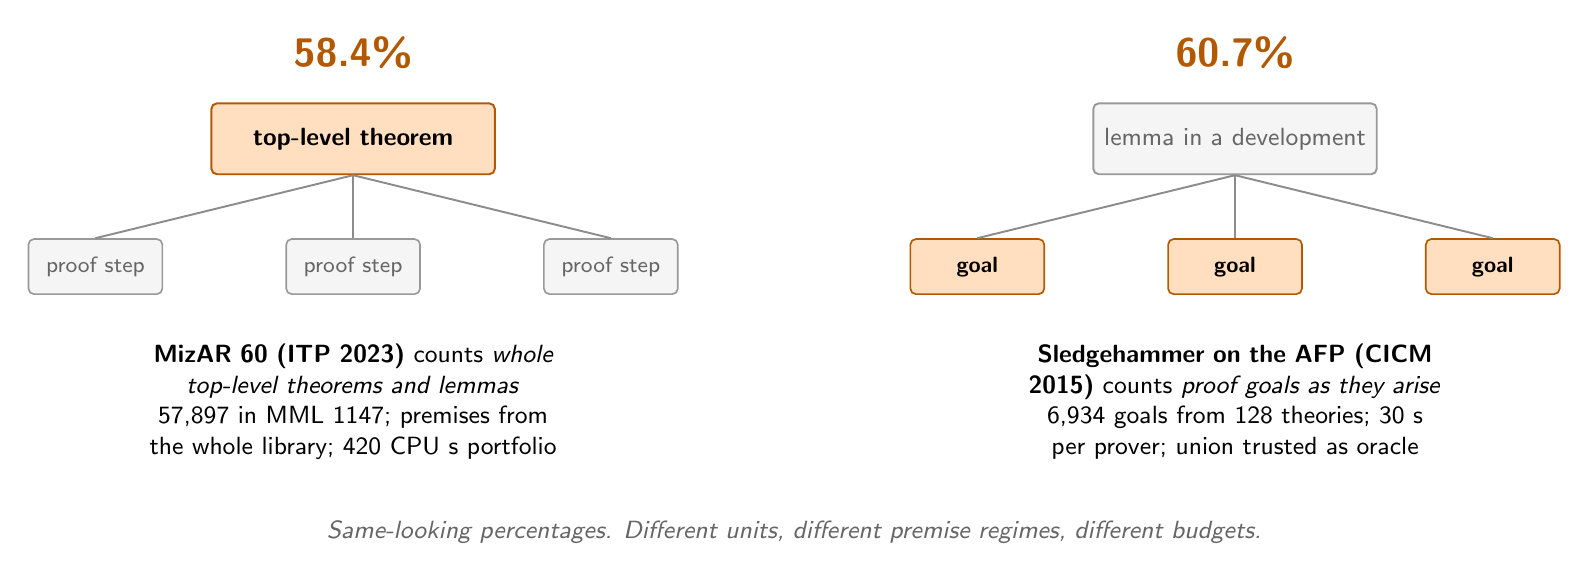
\begin{tikzpicture}[
  font=\sffamily,
  root/.style={draw, rounded corners=2pt, align=center, minimum width=36mm,
               minimum height=9mm, line width=0.7pt, font=\sffamily\small},
  leaf/.style={draw, rounded corners=2pt, align=center, minimum width=17mm,
               minimum height=7mm, line width=0.6pt, font=\sffamily\footnotesize},
  hi/.style={fill=orange!25, draw=orange!70!black},
  lo/.style={fill=black!4, draw=black!40, text=black!60},
  edge/.style={line width=0.7pt, black!45},
  caption/.style={font=\sffamily\small, align=center, text width=70mm},
  big/.style={font=\sffamily\Large\bfseries, align=center, text=orange!70!black},
]
  % MizAR unit: the whole top-level statement
  \node[root, hi] (a) at (0,0) {\textbf{top-level theorem}};
  \node[leaf, lo, below left=8mm and 6mm of a] (a1) {proof step};
  \node[leaf, lo, below=8mm of a] (a2) {proof step};
  \node[leaf, lo, below right=8mm and 6mm of a] (a3) {proof step};
  \foreach \x in {a1,a2,a3} \draw[edge] (a.south) -- (\x.north);
  \node[big, above=3mm of a] {58.4\%};
  \node[caption, below=5mm of a2]
    {\textbf{MizAR 60 (ITP 2023)} counts \emph{whole top-level theorems and lemmas}\\
     57{,}897 in MML 1147; premises from the whole library; 420 CPU s portfolio};

  % AFP unit: goals as they arise
  \node[root, lo] (b) at (112mm,0) {lemma in a development};
  \node[leaf, hi, below left=8mm and 6mm of b] (b1) {\textbf{goal}};
  \node[leaf, hi, below=8mm of b] (b2) {\textbf{goal}};
  \node[leaf, hi, below right=8mm and 6mm of b] (b3) {\textbf{goal}};
  \foreach \x in {b1,b2,b3} \draw[edge] (b.south) -- (\x.north);
  \node[big, above=3mm of b] {60.7\%};
  \node[caption, below=5mm of b2]
    {\textbf{Sledgehammer on the AFP (CICM 2015)} counts \emph{proof goals as they arise}\\
     6{,}934 goals from 128 theories; 30 s per prover; union trusted as oracle};

  \node[font=\sffamily\small\itshape, text=black!60, align=center] at (56mm,-50mm)
    {Same-looking percentages. Different units, different premise regimes, different budgets.};
\end{tikzpicture}
\end{document}
